\documentclass[compress,subsection=false,red,transparent=false]{beamer}


\usepackage{epsf}
%\usepackage{listings}                                                                
\usepackage{tikz}
\usetikzlibrary{arrows,shapes,snakes,automata,backgrounds,petri}
\usepackage{amssymb}
\usepackage{listings}

\mode<presentation>
{


% \usetheme{compatibility}                                                            
%   \setbeamercovered{transparent}                                                    
   \setbeamercovered{invisible}
   \setbeamertemplate{navigation symbols}{}
}

\usepackage[english]{babel}
\usepackage[latin1]{inputenc}
\usepackage{times}
\usepackage[T1]{fontenc}

%\setbeamertemplate{sidebar right}{}                                                  
\newcounter{line}
\setcounter{line}{1}

\usepackage{ifthen}
\usepackage{amssymb}
\newboolean{showcomments}
\setboolean{showcomments}{true}
\ifthenelse{\boolean{showcomments}}
  {\newcommand{\mynote}[2]{
    \fbox{\bfseries\sffamily\scriptsize#1}
    {\small$\blacktriangleright$\textsf{\emph{#2}}$\blacktriangleleft$}
   }
  }
  {\newcommand{\mynote}[2]{}
  }
\newcommand\martin[1]{\mynote{Martin}{#1}}
\newcommand\richard[1]{\mynote{Richard}{#1}}

\newcommand{\NOVSPACEPARAGRAPH}[1]{\NI\textbf{\emph{#1}.}}
\newcommand{\PARAGRAPH}[1]{\vspace{2mm}\NOVSPACEPARAGRAPH{#1}}
\newcommand{\NI}{\noindent}
\newcommand{\LEQ}{\sqsubseteq}
\newcommand{\BISIM}{\sim}
\newcommand{\BIGLUB}{\bigsqcup}
\newenvironment{FIGURE}{\begin{figure}[h]\rule{\linewidth}{0.5pt}
 %\vspace{3.2mm}
}{\rule{\linewidth}{0.5pt}\end{figure}}
\newenvironment{RULES}{\[\begin{array}{c}}{\end{array}\]}
\newenvironment{GRAMMAR}{\[\begin{array}{lcl}}{\end{array}\]}
\newcommand{\VERTICAL}{\  \mid\hspace{-3.0pt}\mid \ }
\newcommand{\infer}[2]{\frac{\displaystyle{ #1 }}{\displaystyle{ #2 }}}
\newcommand{\ZEROPREMISERULE}[1]{\infer{-}{#1}}
\newcommand{\ONEPREMISERULE}[2]{\infer{#1}{#2}}
\newcommand{\TWOPREMISERULE}[3]{\infer{#1 \quad #2}{#3}}
\newcommand{\THREEPREMISERULE}[4]{\infer{#1 \quad #2 \quad #3}{#4}}
\newcommand{\FOURPREMISERULE}[5]{\infer{#1 \quad #2 \quad #3 \quad #4}{#5}}
\newcommand{\SIXPREMISERULE}[7]{\infer{#1 \quad #2 \quad #3 \quad #4 \quad #5 \quad #6}{#7}}
\newcommand{\RULENAME}[1]{\textsc{#1}}
\newcommand{\SMALLRULENAME}[1]{\textsc{\tiny #1}}
\newcommand{\ZEROPREMISERULENAMEDRIGHT}[2]{\ZEROPREMISERULE{#1}\,\SMALLRULENAME{#2}}
\newcommand{\ONEPREMISERULENAMEDRIGHT}[3]{\ONEPREMISERULE{#1}{#2}\,\SMALLRULENAME{#3}}
\newcommand{\TWOPREMISERULENAMEDRIGHT}[4]{\TWOPREMISERULE{#1}{#2}{#3}\,\SMALLRULENAME{#4}}
\newcommand{\THREEPREMISERULENAMEDRIGHT}[5]{\THREEPREMISERULE{#1}{#2}{#3}{#4}\,\SMALLRULENAME{#5}}
\newcommand{\FOURPREMISERULENAMEDRIGHT}[6]{\FOURPREMISERULE{#1}{#2}{#3}{#4}{#5}\,\SMALLRULENAME{#6}}
\newcommand{\ZEROPREMISERULENAMEDLEFT}[2]{\SMALLRULENAME{#2}\,\ZEROPREMISERULE{#1}}
\newcommand{\ONEPREMISERULENAMEDLEFT}[3]{\SMALLRULENAME{#3}\,\ONEPREMISERULE{#1}{#2}}
\newcommand{\TWOPREMISERULENAMEDLEFT}[4]{\SMALLRULENAME{#4}\,\TWOPREMISERULE{#1}{#2}{#3}}
\newcommand{\THREEPREMISERULENAMEDLEFT}[5]{\SMALLRULENAME{#5}\,\THREEPREMISERULE{#1}{#2}{#3}{#4}}
\newcommand{\FOURPREMISERULENAMEDLEFT}[6]{\SMALLRULENAME{#6}\,\FOURPREMISERULE{#1}{#2}{#3}{#4}{#5}}

\newcommand{\MAY}[2]{\langle #1 \rangle #2}
\newcommand{\NEG}[1]{\mathsf{neg}(#1)}
\newcommand{\AND}{\land}
\newcommand{\INC}[1]{\mathsf{Inc}(#1)}

\newcommand{\CAL}[1]{\mathcal{#1}}
\newcommand{\FRAK}[1]{\mathfrak{#1}}
\newcommand{\SEMB}[1]{\lbrack\!\lbrack #1 \rbrack\!\rbrack}
\newcommand{\STATE}{\mathsf{State}}
\newcommand{\SYMBOL}{\mathsf{Symbol}}
\newcommand{\DEFEQ}{\stackrel{\text{\emph{def}}}{=}}
\newcommand{\TRUTH}{\LOGIC{T}}
\newcommand{\TRUE}{\LOGIC{t}}
\newcommand{\LOGIC}[1]{\mathsf{#1}}
\newcommand{\MMM}{\frak{M}}
\newcommand{\SSS}{\CAL{S}}
\newcommand{\IMPLIES}{\supset}
\newcommand{\RED}{\rightarrow}
\newcommand{\RESTRICT}[2]{\mathsf{Restrict}_{#1}(#2)}
\newcommand{\ARROW}[2]{\mathsf{Arrow}(#1, #2)}
\newcommand{\LLL}{\mathcal{L}}
\newcommand{\RRR}{\mathcal{R}}
\newcommand{\TRANS}[1]{\stackrel{#1}{\longrightarrow}}

\newcommand{\QUOTATION}[1]{
\hfill
\hspace{58mm}
\begin{minipage}{60mm}\tiny #1\end{minipage}
}

\lstnewenvironment{code}
    {\lstset{}%
      \csname lst@SetFirstLabel\endcsname}
    {\csname lst@SaveFirstLabel\endcsname}
    \lstset{
      basicstyle=\small\ttfamily,
      flexiblecolumns=false,
      basewidth={0.5em,0.45em},
      literate={+}{{$+$}}1 {/}{{$/$}}1 {*}{{$*$}}1 {=}{{$=$}}1
               {>}{{$>$}}1 {<}{{$<$}}1 {\\}{{$\lambda$}}1
               {\\\\}{{\char`\\\char`\\}}1
               {->}{{$\rightarrow$}}2 {>=}{{$\geq$}}2 {<-}{{$\leftarrow$}}2
               {<=}{{$\leq$}}2 {=>}{{$\Rightarrow$}}2 
               {\ .}{{$\bigcirc$}}2 {\ .\ }{{$\bigcirc$}}2
               {>>}{{>>}}2 {>>=}{{>>=}}2
               {|}{{$\mid$}}1               
    }

\newtheorem{mycase}{Case}
\newtheorem{subcase}{Case}
\numberwithin{subcase}{mycase}


% Dot
\def\fDot {\ast}
% Bang
\def\fBang {\ ! \ }
% Or
\def\fOr {\ | \ }

% Turnstiles with subscripts
\def\judgeX {\sststile{\mathrm{X}}{}}
\def\judgeY {\sststile{\mathrm{Y}}{}}
%\def\judge {\sststile{\mathrm{}}{}}

\newcommand{\judge}{\vdash}

\EnableBpAbbreviations


\setbeamertemplate{footline}[text line]{%
  \parbox{\linewidth}{\vspace*{-8pt}\hfill\insertpagenumber}}
\setbeamertemplate{navigation symbols}{}


\title{Cathoristic Logic}
\subtitle{A Modal Logic of Incompatible Propositions}
\author{Richard Prideaux Evans (DeepMind \& Imperial) \\ Martin Berger (Sussex)}
\date{18 September 2019}

\begin{document}





%% %%%%%%%%%%%%%%%%%%%%%%% file typeinst.tex %%%%%%%%%%%%%%%%%%%%%%%%%
%% %
%% % This is the LaTeX source for the instructions to authors using
%% % the LaTeX document class 'llncs.cls' for contributions to
%% % the Lecture Notes in Computer Sciences series.
%% % http://www.springer.com/lncs       Springer Heidelberg 2006/05/04
%% %
%% % It may be used as a template for your own input - copy it
%% % to a new file with a new name and use it as the basis
%% % for your article.
%% %
%% % NB: the document class 'llncs' has its own and detailed documentation, see
%% % ftp://ftp.springer.de/data/pubftp/pub/tex/latex/llncs/latex2e/llncsdoc.pdf
%% %
%% %%%%%%%%%%%%%%%%%%%%%%%%%%%%%%%%%%%%%%%%%%%%%%%%%%%%%%%%%%%%%%%%%%%


%% \documentclass{beamer}

%% \usepackage{amssymb}
%% \setcounter{tocdepth}{3}
%% \usepackage{graphicx}
%% \usepackage{color}

%% \usepackage{url}
%% \urldef{\mailsa}\path|richarde@maxis.com|

%% \usepackage{amsmath}
%% \usepackage{listings}
%% \usepackage{subfig}
%% %\usepackage{bussproofs}
%% %\usepackage{amsthm}
%% \usepackage{pgf}
%% \usepackage{tikz}
%% \usetikzlibrary{arrows,shapes,snakes,automata,backgrounds,petri}
%% \usepackage[latin1]{inputenc}
%% \usepackage{float}
%% \usepackage{amssymb}

%% \usepackage{ifthen}
\usepackage{amssymb}
\newboolean{showcomments}
\setboolean{showcomments}{true}
\ifthenelse{\boolean{showcomments}}
  {\newcommand{\mynote}[2]{
    \fbox{\bfseries\sffamily\scriptsize#1}
    {\small$\blacktriangleright$\textsf{\emph{#2}}$\blacktriangleleft$}
   }
  }
  {\newcommand{\mynote}[2]{}
  }
\newcommand\martin[1]{\mynote{Martin}{#1}}
\newcommand\richard[1]{\mynote{Richard}{#1}}

\newcommand{\NOVSPACEPARAGRAPH}[1]{\NI\textbf{\emph{#1}.}}
\newcommand{\PARAGRAPH}[1]{\vspace{2mm}\NOVSPACEPARAGRAPH{#1}}
\newcommand{\NI}{\noindent}
\newcommand{\LEQ}{\sqsubseteq}
\newcommand{\BISIM}{\sim}
\newcommand{\BIGLUB}{\bigsqcup}
\newenvironment{FIGURE}{\begin{figure}[h]\rule{\linewidth}{0.5pt}
 %\vspace{3.2mm}
}{\rule{\linewidth}{0.5pt}\end{figure}}
\newenvironment{RULES}{\[\begin{array}{c}}{\end{array}\]}
\newenvironment{GRAMMAR}{\[\begin{array}{lcl}}{\end{array}\]}
\newcommand{\VERTICAL}{\  \mid\hspace{-3.0pt}\mid \ }
\newcommand{\infer}[2]{\frac{\displaystyle{ #1 }}{\displaystyle{ #2 }}}
\newcommand{\ZEROPREMISERULE}[1]{\infer{-}{#1}}
\newcommand{\ONEPREMISERULE}[2]{\infer{#1}{#2}}
\newcommand{\TWOPREMISERULE}[3]{\infer{#1 \quad #2}{#3}}
\newcommand{\THREEPREMISERULE}[4]{\infer{#1 \quad #2 \quad #3}{#4}}
\newcommand{\FOURPREMISERULE}[5]{\infer{#1 \quad #2 \quad #3 \quad #4}{#5}}
\newcommand{\SIXPREMISERULE}[7]{\infer{#1 \quad #2 \quad #3 \quad #4 \quad #5 \quad #6}{#7}}
\newcommand{\RULENAME}[1]{\textsc{#1}}
\newcommand{\SMALLRULENAME}[1]{\textsc{\tiny #1}}
\newcommand{\ZEROPREMISERULENAMEDRIGHT}[2]{\ZEROPREMISERULE{#1}\,\SMALLRULENAME{#2}}
\newcommand{\ONEPREMISERULENAMEDRIGHT}[3]{\ONEPREMISERULE{#1}{#2}\,\SMALLRULENAME{#3}}
\newcommand{\TWOPREMISERULENAMEDRIGHT}[4]{\TWOPREMISERULE{#1}{#2}{#3}\,\SMALLRULENAME{#4}}
\newcommand{\THREEPREMISERULENAMEDRIGHT}[5]{\THREEPREMISERULE{#1}{#2}{#3}{#4}\,\SMALLRULENAME{#5}}
\newcommand{\FOURPREMISERULENAMEDRIGHT}[6]{\FOURPREMISERULE{#1}{#2}{#3}{#4}{#5}\,\SMALLRULENAME{#6}}
\newcommand{\ZEROPREMISERULENAMEDLEFT}[2]{\SMALLRULENAME{#2}\,\ZEROPREMISERULE{#1}}
\newcommand{\ONEPREMISERULENAMEDLEFT}[3]{\SMALLRULENAME{#3}\,\ONEPREMISERULE{#1}{#2}}
\newcommand{\TWOPREMISERULENAMEDLEFT}[4]{\SMALLRULENAME{#4}\,\TWOPREMISERULE{#1}{#2}{#3}}
\newcommand{\THREEPREMISERULENAMEDLEFT}[5]{\SMALLRULENAME{#5}\,\THREEPREMISERULE{#1}{#2}{#3}{#4}}
\newcommand{\FOURPREMISERULENAMEDLEFT}[6]{\SMALLRULENAME{#6}\,\FOURPREMISERULE{#1}{#2}{#3}{#4}{#5}}

\newcommand{\MAY}[2]{\langle #1 \rangle #2}
\newcommand{\NEG}[1]{\mathsf{neg}(#1)}
\newcommand{\AND}{\land}
\newcommand{\INC}[1]{\mathsf{Inc}(#1)}

\newcommand{\CAL}[1]{\mathcal{#1}}
\newcommand{\FRAK}[1]{\mathfrak{#1}}
\newcommand{\SEMB}[1]{\lbrack\!\lbrack #1 \rbrack\!\rbrack}
\newcommand{\STATE}{\mathsf{State}}
\newcommand{\SYMBOL}{\mathsf{Symbol}}
\newcommand{\DEFEQ}{\stackrel{\text{\emph{def}}}{=}}
\newcommand{\TRUTH}{\LOGIC{T}}
\newcommand{\TRUE}{\LOGIC{t}}
\newcommand{\LOGIC}[1]{\mathsf{#1}}
\newcommand{\MMM}{\frak{M}}
\newcommand{\SSS}{\CAL{S}}
\newcommand{\IMPLIES}{\supset}
\newcommand{\RED}{\rightarrow}
\newcommand{\RESTRICT}[2]{\mathsf{Restrict}_{#1}(#2)}
\newcommand{\ARROW}[2]{\mathsf{Arrow}(#1, #2)}
\newcommand{\LLL}{\mathcal{L}}
\newcommand{\RRR}{\mathcal{R}}
\newcommand{\TRANS}[1]{\stackrel{#1}{\longrightarrow}}

\newcommand{\QUOTATION}[1]{
\hfill
\hspace{58mm}
\begin{minipage}{60mm}\tiny #1\end{minipage}
}

\lstnewenvironment{code}
    {\lstset{}%
      \csname lst@SetFirstLabel\endcsname}
    {\csname lst@SaveFirstLabel\endcsname}
    \lstset{
      basicstyle=\small\ttfamily,
      flexiblecolumns=false,
      basewidth={0.5em,0.45em},
      literate={+}{{$+$}}1 {/}{{$/$}}1 {*}{{$*$}}1 {=}{{$=$}}1
               {>}{{$>$}}1 {<}{{$<$}}1 {\\}{{$\lambda$}}1
               {\\\\}{{\char`\\\char`\\}}1
               {->}{{$\rightarrow$}}2 {>=}{{$\geq$}}2 {<-}{{$\leftarrow$}}2
               {<=}{{$\leq$}}2 {=>}{{$\Rightarrow$}}2 
               {\ .}{{$\bigcirc$}}2 {\ .\ }{{$\bigcirc$}}2
               {>>}{{>>}}2 {>>=}{{>>=}}2
               {|}{{$\mid$}}1               
    }

\newtheorem{mycase}{Case}
\newtheorem{subcase}{Case}
\numberwithin{subcase}{mycase}


% Dot
\def\fDot {\ast}
% Bang
\def\fBang {\ ! \ }
% Or
\def\fOr {\ | \ }

% Turnstiles with subscripts
\def\judgeX {\sststile{\mathrm{X}}{}}
\def\judgeY {\sststile{\mathrm{Y}}{}}
%\def\judge {\sststile{\mathrm{}}{}}

\newcommand{\judge}{\vdash}

\EnableBpAbbreviations



%% \usetheme{Montpellier}


%% \begin{document}

\begin{frame}
\titlepage
\end{frame}

\begin{frame}{October 1994}

  \pause
  MB: What is a type, abstractly? 


  \VSPACE\pause
  CH: I don't know.
\end{frame}


\begin{frame}{25 years later}

    I still  don't understand the concept of types abstractly.

\end{frame}

\begin{frame}

\includegraphics[height=9cm]{images/barbie1.jpg}  
\end{frame}



\begin{frame}
What's the  second most boring and simple thing in logic?

\pause
\VSPACE

\[
   A \quad ::= \quad ... \VERTICAL \neg A
\]

\end{frame}

\begin{frame}{  Isn't negation solved?}

  \pause
  \VSPACE
  No
\end{frame}

\begin{frame}{Problem with negation}
    \pause
  \begin{itemize}

    \item Computational complexity (query complexity in DB queries, see \url{http://www.versu.com} for a use case)

    \item Philosophy (Hegel, Sellars, Brandom)

  \end{itemize}

  \VSPACE
  \pause
  Cathoristic logic came out the need to use the latter for the former!
\end{frame}

\begin{frame}{Problem with negation: query complexity}
      \pause

    \begin{center}
    
\includegraphics[height=7cm]{images/fire.jpg}
  \end{center}
\end{frame}


\begin{frame}[fragile]{Problem with negation: query complexity}

  Let $P$ be the following predicate:
\begin{verbatim}
  SELECT * FROM HumanDB WHERE
     name = ``Martin Berger''
     knowsPiCalculus = true
     personality = ``obnoxious''
\end{verbatim}

\VSPACE\pause
1 inhabitant


\VSPACE\pause
Negation
\[
\neg P
\]

\VSPACE\pause
> 7 billion  inhabitants

\end{frame}


\begin{frame}[fragile]{Core insight}

  \VSPACE\pause
  In many situations, we want / need to express only:

  \begin{verbatim}
    x is: this, that, the other
\end{verbatim}

  \VSPACE\pause
  Of course you can specify this in FOL, but ... needs too much power
\end{frame}


\begin{frame}
Simplify simplify simplify
\end{frame}


\begin{frame}
  Replace negation with a predicate of 'this that the other', which
  \EMPH{lists} all possibilities:
  \[
    \{opt_1, ..., opt_n\}
  \]
\end{frame}

\begin{frame}
  Let's add this to a logic!

  \VSPACE\pause

  What's a simplest interesting logic?

\VSPACE\pause

Hennessy-Milner logic:
\begin{GRAMMAR}
  \phi 
     &\quad ::= \quad & 
  \TRUE 
     \VERTICAL 
  \phi \AND \psi
     \VERTICAL 
  \MAY{a}{\phi}
     \VERTICAL 
  \textcolor{blue}{\neg \phi}
\end{GRAMMAR}
\pause
\Cathoristic{}:
\begin{GRAMMAR}
  \phi 
     &\quad ::= \quad & 
  \TRUE 
     \VERTICAL 
  \phi \AND \psi
     \VERTICAL 
  \MAY{a}{\phi}
     \VERTICAL 
  \textcolor{red}{\fBang A}
\end{GRAMMAR}

  \VSPACE\pause

``Cathoristic'' comes from the Greek
  $\kappa \alpha \theta o \rho \acute{\i} \zeta \epsilon i \nu$: to impose narrow
  boundaries.

\end{frame}

\section{Demo}
%% \begin{frame}
%% \begin{itemize}
%% \item
%% \Cathoristic{} is used in a multi-agent simulation
%% \item
%% Thousands of rules 
%% \item
%% Tens of thousands of facts
%% \item
%% Demo!
%% \end{itemize}
%% \end{frame}


  
\begin{frame}{Syntax}
\textcolor{red}{\Cathoristic{}} is a multi-modal logic with one new operator:
\begin{GRAMMAR}
  \phi 
     &\quad ::= \quad & 
  \TRUE 
     \VERTICAL 
  \phi \AND \psi
     \VERTICAL 
  \MAY{a}{\phi}
     \VERTICAL 
  \textcolor{red}{\fBang A }
\end{GRAMMAR}
Here:
\begin{itemize}
\item
$\Sigma$ is a set of actions
\item
$a$ ranges over  $\Sigma$
\item
$A$ ranges over subsets of  $\Sigma$
\end{itemize}
$\fBang A$ means the \EMPH{only} transitions allowed are those specified in $A$.

\VSPACE\pause
$!A$ is pronounced  ``Tantum'' (Latin for ``only'').
\end{frame}

\begin{frame}{Comparing with Hennessy-Milner Logic}
Hennessy-Milner logic:
\begin{GRAMMAR}
  \phi 
     &\quad ::= \quad & 
  \TRUE 
     \VERTICAL 
  \phi \AND \psi
     \VERTICAL 
  \MAY{a}{\phi}
     \VERTICAL 
  \textcolor{blue}{\neg \phi}
\end{GRAMMAR}
\Cathoristic{}:
\begin{GRAMMAR}
  \phi 
     &\quad ::= \quad & 
  \TRUE 
     \VERTICAL 
  \phi \AND \psi
     \VERTICAL 
  \MAY{a}{\phi}
     \VERTICAL 
  \textcolor{red}{\fBang A}
\end{GRAMMAR}
Note:
\begin{itemize}
\item
\textcolor{red}{\Cathoristic{} does not have negation}
\item
Hence no disjunction, implication, $\MUST{a}$, etc
\item
  Instead, it has the $\fBang$ operator

\item DeMorgan duality is \EMPH{not} available. So definability of
  disjunction, implication, $\MUST{a}$, etc is ... subtle
\end{itemize}
\end{frame}


\begin{frame}{Examples of the $\fBang$ Operator}
The \EMPH{only} colours the traffic light can be are green, amber or red:
\[
\fBang \{green, amber, red\}
\]
\end{frame}

\begin{frame}{Examples of the $\fBang$ Operator}
The traffic light is amber and amber is its \EMPH{only} colour:
\[
\MAY{amber} \land \fBang\{amber\}
\]
Pierre is the (unique) King of France:
\[
\MAY{king}\MAY{france}(\MAY{pierre} \land \fBang \{pierre\})
\]
\end{frame}


\begin{frame}{Comparing With FOL}
First-order logic with identity:
\[
king(france, pierre) \land (\forall x) king(france, x) \rightarrow x = pierre
\]
\Cathoristic{}:
\[
\MAY{king}\MAY{france}(\MAY{pierre} \land \fBang \{pierre\})
\]
\end{frame}


\begin{frame}{Incompatibility Without Negation}
Even though \cathoristic{} has no negation, it can express \EMPH{incompatible} statements:
\begin{eqnarray*}
\fBang \{green, amber, red\} \\
\MAY{blue}
\end{eqnarray*}
There is no model in which both these statements are true. 
\end{frame}



\begin{frame}{Motivation}
The following sentences cannot both be true:
\begin{itemize}
\item
Jack is male
\item
Jack is female
\end{itemize}
\EMPH{Why} are these sentences incompatible?
\end{frame}

\begin{frame}{Incompatibility in First-Order Logic}
``Jack is male'' is incompatible with ``Jack is female'' because:
\[
(\forall x) male(x) \rightarrow \neg female(x)
\]
In \fol{}, incompatibility is explained in terms of:
\begin{enumerate}
\item
Universal quantification (including $\alpha$-conversion ... oh my)
\item
Implication
\item
  \EMPH{Negation}


\end{enumerate}
\end{frame}


\begin{frame}{An Alternative Understanding of Incompatibility}
``Jack is male'' is incompatible with ``Jack is female'' because:
\begin{quote}
``\_ is male'' and ``\_ is female'' are \EMPH{incompatible predicates}
\end{quote}
Philosophical claim: We can understand incompatible predicates even if
we do not understand quantification, implication or negation.
\end{frame}

\begin{frame}{Intuition from the philosophy of language}
  \pause
  Imagine: a primitive people speaking a primordial language
  \VSPACE
\begin{itemize}

\pause\item Including incompatible predicates ``gooda'' and ``bada''
\pause\item They can express sentences that \EMPH{are} incompatible
\pause\item But they cannot express \EMPH{that} they are incompatible
\end{itemize}

\VSPACE
Their language is \EMPH{just fine}!


\end{frame}

\begin{frame}{Intuition from the philosophy of language}
Now:
\begin{itemize}
\item
Later, they \EMPH{may} enrich their language with an explicit negation operator
\item
But this is an \EMPH{optional} development
\item
Their language was \EMPH{just fine} before the addition of negation
\end{itemize}

\end{frame}

\begin{frame}{Intuition from the philosophy of language}
Imagine:
\begin{itemize}
\item
A primitive people speaking a primordial language
\item
Including incompatible predicates ``gooda'' and ``bada''
\item
They can express sentences that \EMPH{are} incompatible
\item
But they cannot express \EMPH{that} they are incompatible
\end{itemize}
If this is possible, then \textcolor{red}{incompatibility is conceptually independent of negation}.
\end{frame} 

\begin{frame}<beamer:0>
Now imagine an alternative in which:
\begin{itemize}
\item
The people do not treat \EMPH{any} sentences as incompatible
\item 
If Jack says that Bob is ``gooda'' and Jill says that he is ``bada'', there is no sense of \EMPH{conflict, disagreement, challenge}.
\item
In this case, there is not enough structure for this practice to count as a \EMPH{language}.
\end{itemize}
If this does not count as a language, then incompatibility is not just \EMPH{independent} of negation.
\textcolor{red}{Incompatibility might be \EMPH{conceptually prior} to negation.}
\end{frame}

\begin{frame}
An alternative understanding of the relation between incompatibility and negation:
\begin{itemize}
\item
Incompatibility might be conceptually prior to negation
\item
Brandom follows Sellars follows Hegel
\item
  Hegel's word for incompatibility is ``determinate negation'' (German: ``bestimmte Negation'').
  Brandom called ``determinate negation'' Hegel's most fundamental conceptual tool. 
\item
\Cathoristic{} is the simplest logic we could find that respects this alternative direction of explanation
\end{itemize}
\end{frame}



\begin{frame}{Wittgenstein on Incompatibility}
In the \EMPH{Tractatus}:
\begin{itemize}
\item
The world is a set of atomic sentences in a logical language
\item
Each atomic sentence was supposed to be logically independent of every other...
\item
...so that they can be combined in every possible permutation, willy-nilly
\end{itemize}
\end{frame}

\begin{frame}
But Wittgenstein was aware of many counterexamples to this idea:
\begin{quote}
For two colours, e.g., to be at one place in the visual field is impossible, and indeed logically impossible, for it is excluded by the logical structure of colour. (6.3751)
\end{quote}
\end{frame}

\begin{frame}
Later, in the \EMPH{Philosophical Remarks}, Wittgenstein renounced the thesis of the logical independence of atomic propositions:
\begin{quote}
That makes it look as if a construction might be possible within the elementary proposition. That is to say, \EMPH{as if there were a construction in logic which didn't work by means of truth functions}. What's more, it also seems that these constructions have an effect on one proposition's following logically from another. For, if different degrees exclude one another it follows from the presence of one that the other is not present. In that case, \textcolor{red}{two elementary propositions can contradict one another}.
\end{quote}
\end{frame}



\begin{frame}{Additional Property of Cathoristic Logic: Inferences Between Atomic Sentences}
The \EMPH{atomic sentences} are those sentences that do not contain other sentences as constituent parts:
\begin{itemize}
\item
Jack is male
\item
Jack loves Jill
\item
Jack and Jill are bruised
\end{itemize}
\end{frame}

\begin{frame}
The following are not atomic:
\begin{itemize}
\item
Jack is bruised and Jill is annoyed
\item
Jack knows that Jill is annoyed
\end{itemize}
\end{frame}

\begin{frame}
Now:
\begin{itemize}
\item
The incompatibility between ``Jack is male'' and ``Jack is female'' is a logical relation between \EMPH{atomic sentences}.
\item
Are there any \EMPH{other} logical relations between atomic sentences?
\end{itemize}
\end{frame}

\begin{frame}
Other logical relations between atomic sentences:
\begin{itemize}
\item
``Jill is annoyed with Jack'' implies ``Jill is annoyed''
\item
``Jack walks slowly'' implies ``Jack walks''
\item
``Jack loves Jill''  and ``Jack loves Joan'' together imply that ``Jack loves Jill and Joan''
\item
``Jack is bruised and humiliated'' implies ``Jack is humiliated''
\end{itemize}
\Cathoristic{} is the simplest logic we could find that captures these inferences between atomic sentences.
\end{frame}

\begin{frame}{Semantics}
\end{frame}

\begin{frame}{Recall: Syntax}
\Cathoristic{}:
\begin{GRAMMAR}
  \phi 
     &\quad ::= \quad & 
  \TRUE 
     \VERTICAL 
  \phi \AND \psi
     \VERTICAL 
  \MAY{a}{\phi}
     \VERTICAL 
  \fBang A 
\end{GRAMMAR}
Here:
\begin{itemize}
\item
$\Sigma$ is a set of actions
\item
$a$ ranges over  $\Sigma$
\item
$A$ ranges over subsets of  $\Sigma$
\end{itemize}
$\fBang A$ means the \EMPH{only} transitions allowed are those specified in $A$.
\end{frame}

\begin{frame}{Semantics}
Preliminaries:
\begin{itemize}
\item
Let $\Sigma$ be a set of \EMPH{actions}.  
\item
A \EMPH{labelled transition
  system over $\Sigma$} is a pair $(\mathcal{S}, \rightarrow)$ where
\begin{itemize}
\item
$\mathcal{S}$ is a set of \EMPH{states} 
\item
$\rightarrow \subseteq
\mathcal{S} \times \Sigma \times \mathcal{S}$ is the \EMPH{transition
  relation}.  
\end{itemize}
\item
 We write $x \xrightarrow{a} y$ to abbreviate $(x,a,y)
\in \rightarrow$. 
\item
We say $\LLL$ is \EMPH{deterministic} if $x \TRANS{a} y$ and
$x \TRANS{a} z$ imply that $y = z$. 
\end{itemize}
\end{frame}

\begin{frame}
A \textcolor{red}{cathoristic transition system} is a triple $\LLL = (S,
\rightarrow, \lambda)$, where $(S, \rightarrow)$ is a \EMPH{deterministic}
labelled transition system over $\Sigma$, and $\lambda$ is a function
from states to sets of actions (not necessarily finite), subject to
the following constraints:
\begin{itemize}

\item For all states $s \in S$ it is the case that $ \{a \fOr \exists
  t \; s \xrightarrow{a} t\} \subseteq \lambda(s)$. We call this
  condition \EMPH{admissibility}.

\item For all states $s \in S$, $\lambda (s)$ is either finite or
  $\Sigma$. We call this condition \EMPH{well-sizedness}.

\end{itemize}
\end{frame}

\begin{frame}
In $\LLL = (S,\rightarrow, \lambda)$:
\begin{itemize}
\item
$\lambda(w)$ is the set of
allowed actions emanating from $w$.  
\item
The $\lambda$ function
is the semantic counterpart of the $!$ operator.  
\item
The admissibility
restriction rules out the case where $s \TRANS{a} t$ but $a
\notin \lambda(s)$. This case would be saying that an $a$ action is possible at
$s$ but at the same time prohibited at $s$.
\end{itemize}
\end{frame}

\begin{frame}
A \textcolor{red}{cathoristic model} is a pair $(\LLL, s)$:
\begin{itemize}
\item
$\LLL$ is a cathoristic transition system $(S,
\rightarrow, \lambda)$
\item
$s \in S$ is the \EMPH{start state} of the model
\end{itemize}
\end{frame}

\begin{frame}
Satisfaction of a formula $\phi$ is defined relative to a cathoristic model $\MMM$:
\[
\begin{array}{lclcl}
  \MMM & \models & \top   \\
  \MMM & \models & \phi \AND \psi &\ \mbox{ iff } \ & \MMM  \models \phi \mbox { and } \MMM \models \psi  \\
  \MMM & \models & \langle a \rangle \phi & \mbox{ iff } & \text{there is transition } s \xrightarrow{a} t \mbox { such that } (\LLL, t) \models \phi  \\
  \MMM & \models & \fBang A &\mbox{ iff } & \lambda(s) \subseteq A
\end{array}
\]
Here, we assume that $\MMM =
(\LLL, s)$ and $\LLL = (S, \rightarrow, \lambda)$.
\end{frame}

\begin{frame}
\begin{FIGURE}
\centering
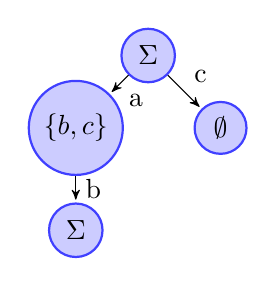
\begin{tikzpicture}[node distance=1.3cm,>=stealth',bend angle=45,auto]
  \tikzstyle{place}=[circle,thick,draw=blue!75,fill=blue!20,minimum size=6mm]
  \tikzstyle{red place}=[place,draw=red!75,fill=red!20]
  \tikzstyle{transition}=[rectangle,thick,draw=black!75,
  			  fill=black!20,minimum size=4mm]
  \tikzstyle{every label}=[red]
  
  \begin{scope}
    \node [place] (w1) {$\Sigma$};
    \node [place] (e1) [below left of=w1] {$\{b,c\}$}
      edge [pre]  node[swap] {a}                 (w1);      
    \node [place] (e2) [below right of=w1] {$\emptyset$}
      edge [pre]  node[swap] {c}                 (w1);      
    \node [place] (e3) [below of=e1] {$\Sigma$}
      edge [pre]  node[swap] {b}                 (e1);      
  \end{scope}
    
\end{tikzpicture}
\caption{Example model.}\label{figure:elSmall}
\end{FIGURE}


The model satisfies the following formulae, amongst
others:
\[
\begin{array}{lclclclcl}
\MAY{a} &\qquad&
\MAY{a} \MAY{b} &\qquad&
\MAY{a} \fBang \{b,c\} &\qquad&
\MAY{a} \fBang \{b,c,d\} \\[1mm]
\MAY{c} \fBang \emptyset &&
\MAY{c} \fBang \{a\} &&
\MAY{c} \fBang \{a,b\} &&
\MAY{a} (\MAY{b} \land \fBang \{b,c\}
\end{array}
\]
\end{frame}

\begin{frame}
\begin{FIGURE}
\centering
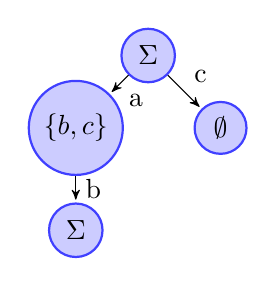
\begin{tikzpicture}[node distance=1.3cm,>=stealth',bend angle=45,auto]
  \tikzstyle{place}=[circle,thick,draw=blue!75,fill=blue!20,minimum size=6mm]
  \tikzstyle{red place}=[place,draw=red!75,fill=red!20]
  \tikzstyle{transition}=[rectangle,thick,draw=black!75,
  			  fill=black!20,minimum size=4mm]
  \tikzstyle{every label}=[red]
  
  \begin{scope}
    \node [place] (w1) {$\Sigma$};
    \node [place] (e1) [below left of=w1] {$\{b,c\}$}
      edge [pre]  node[swap] {a}                 (w1);      
    \node [place] (e2) [below right of=w1] {$\emptyset$}
      edge [pre]  node[swap] {c}                 (w1);      
    \node [place] (e3) [below of=e1] {$\Sigma$}
      edge [pre]  node[swap] {b}                 (e1);      
  \end{scope}
    
\end{tikzpicture}
\caption{Example model.}\label{figure:elSmall}
\end{FIGURE}


The same model does not satisfy any of the following formulae:
\[
\MAY{b} \qquad
\fBang \{a\} \qquad
\fBang \{a, c\} \qquad
\MAY{a} \fBang \{b\} \qquad
\MAY{a} \MAY{c} \qquad
\MAY{a} \MAY{b} \fBang \{c\} 
\]

\end{frame}

\begin{frame}
\begin{FIGURE}
\centering
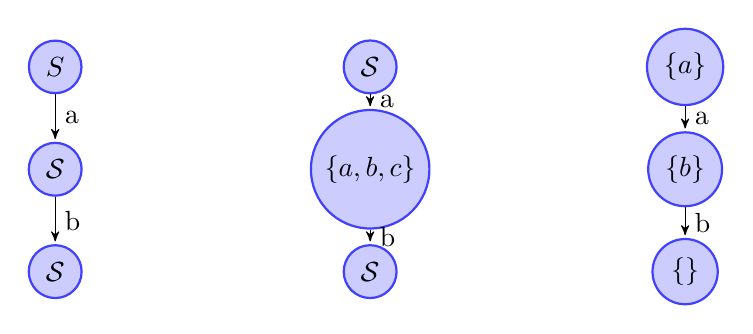
\begin{tikzpicture}[node distance=1.3cm,>=stealth',bend angle=45,auto]
  \tikzstyle{place}=[circle,thick,draw=blue!75,fill=blue!20,minimum size=6mm]
  \tikzstyle{red place}=[place,draw=red!75,fill=red!20]
  \tikzstyle{transition}=[rectangle,thick,draw=black!75,
  			  fill=black!20,minimum size=4mm]
  \tikzstyle{every label}=[red]
  \begin{scope}[xshift=0cm]
    \node [place] (w1) {$S$};
    \node [place] (e1) [below of=w1] {$\mathcal{S}$}
      edge [pre]  node[swap] {a}                 (w1);
    \node [place] (e2) [below of=e1] {$\mathcal{S}$}
      edge [pre]  node[swap] {b}                 (e1);
  \end{scope}   
  \begin{scope}[xshift=4cm]
    \node [place] (w1) {$\mathcal{S}$};
    \node [place] (e1) [below of=w1] {$\{a,b,c\}$}
      edge [pre]  node[swap] {a}                 (w1);
    \node [place] (e2) [below of=e1] {$\mathcal{S}$}
      edge [pre]  node[swap] {b}                 (e1);
  \end{scope}   
  \begin{scope}[xshift=8cm]
    \node [place] (w1) {$\{a\}$};
    \node [place] (e1) [below of=w1] {$\{b\}$}
      edge [pre]  node[swap] {a}                 (w1);
    \node [place] (e2) [below of=e1] {$\{\}$}
      edge [pre]  node[swap] {b}                 (e1);
  \end{scope}   
\end{tikzpicture}
\caption{Various models of $\langle a \rangle \langle b \rangle \top$}
\end{FIGURE}

\end{frame}

\begin{frame}
As \cathoristic{} does not have the $\neg, \lor, \rightarrow$ operators:
\begin{itemize}
\item
Each formula has a unique simplest model
\item
There are no tautologies (apart from $\top$)
\item
But there are an infinite number of contradictories
\end{itemize}
\end{frame}

\begin{frame}
Each formula has a unique simplest model:
\begin{FIGURE}
\centering
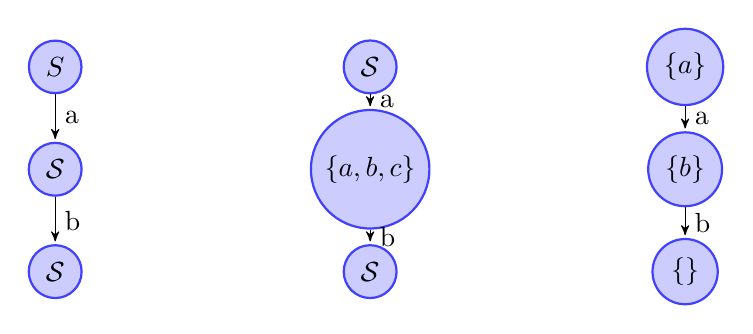
\begin{tikzpicture}[node distance=1.3cm,>=stealth',bend angle=45,auto]
  \tikzstyle{place}=[circle,thick,draw=blue!75,fill=blue!20,minimum size=6mm]
  \tikzstyle{red place}=[place,draw=red!75,fill=red!20]
  \tikzstyle{transition}=[rectangle,thick,draw=black!75,
  			  fill=black!20,minimum size=4mm]
  \tikzstyle{every label}=[red]
  \begin{scope}[xshift=0cm]
    \node [place] (w1) {$S$};
    \node [place] (e1) [below of=w1] {$\mathcal{S}$}
      edge [pre]  node[swap] {a}                 (w1);
    \node [place] (e2) [below of=e1] {$\mathcal{S}$}
      edge [pre]  node[swap] {b}                 (e1);
  \end{scope}   
  \begin{scope}[xshift=4cm]
    \node [place] (w1) {$\mathcal{S}$};
    \node [place] (e1) [below of=w1] {$\{a,b,c\}$}
      edge [pre]  node[swap] {a}                 (w1);
    \node [place] (e2) [below of=e1] {$\mathcal{S}$}
      edge [pre]  node[swap] {b}                 (e1);
  \end{scope}   
  \begin{scope}[xshift=8cm]
    \node [place] (w1) {$\{a\}$};
    \node [place] (e1) [below of=w1] {$\{b\}$}
      edge [pre]  node[swap] {a}                 (w1);
    \node [place] (e2) [below of=e1] {$\{\}$}
      edge [pre]  node[swap] {b}                 (e1);
  \end{scope}   
\end{tikzpicture}
\caption{Various models of $\langle a \rangle \langle b \rangle \top$}
\end{FIGURE}

\end{frame}

\begin{frame}
There are an infinite number of contradictories:
\[
   \MAY{a} \;\land\; \fBang \emptyset \qquad
   \MAY{a} \;\land\; \fBang \{b\} \qquad
   \MAY{a} \;\land\; \fBang \{b, c\} \qquad
   \MAY{b} \;\land\; \fBang \emptyset \qquad
\]
\end{frame}


\begin{frame}{Implication}
We say $\phi$ \textcolor{red}{semantically implies} $\psi$, written $\phi \models \psi$, iff for every cathoristic model $\MMM$, if  $\MMM \models \phi$, then $\MMM \models \psi$.
\end{frame}

\begin{frame}
Cathoristic logic shares with Hennessy-Milner logic the following implications:
\begin{itemize}
\item
$\MAY{a} \MAY{b} \models \MAY{a}$
\item
$\MAY{a} (\MAY{b} \land \MAY{c}) \models \MAY{a} \MAY{b}$
\end{itemize}
\end{frame}

\begin{frame}
As \cathoristic{} is restricted to \EMPH{deterministic} models:
\begin{eqnarray*}
\MAY{a} \MAY{b} \land \MAY{a} \MAY{c}  \models \MAY{a} (\MAY{b} \land \MAY{c})
\end{eqnarray*}
This formula is \EMPH{not} valid in Hennessy-Milner logic.
\end{frame}

\begin{frame}
\Cathoristic{} also validates all implications in which the set of constraints is relaxed from left to right:
\begin{eqnarray*}
\fBang \{c\} \models\ \fBang \{a, b, c\} 
 \qquad\qquad
\fBang \emptyset \models\ \fBang \{a, b\} 
\end{eqnarray*}
\end{frame}

\begin{frame}
\Cathoristic{} also validates all implications in which the antecedent involves an incompatible conjunction:
\begin{eqnarray*}
\MAY{a} \land \fBang \{b\} & \models & \MAY{c} \\
\MAY{a} \land \fBang \{\} & \models & \fBang \{b\}
\end{eqnarray*}
\end{frame}

\section{Inferences Between Atomic Sentences}

\begin{frame}
\Cathoristic{} can capture the following logical inferences between atomic sentences:
\begin{itemize}
\item
``Jack is male'' is incompatible with ``Jack is female''
\item
``Jill is annoyed with Jack'' implies ``Jill is annoyed''
\item
``Jack walks slowly'' implies ``Jack walks''
\item
``Jack loves Jill''  and ``Jack loves Joan'' together imply that ``Jack loves Jill and Joan''
\item
``Jack is bruised and humiliated'' implies ``Jack is humiliated''
\end{itemize}
\end{frame}

\begin{frame}{Incompatibility}
``Jack is male'' is incompatible with ``Jack is female'':
\begin{eqnarray*}
\MAY{jack}\MAY{sex}(\MAY{male} \land \fBang \{male\}) \\
\MAY{jack}\MAY{sex}(\MAY{female} \land \fBang \{female\})
\end{eqnarray*}
There is no model which satisfies both of these formulae.
\end{frame}

\begin{frame}{Inferences from Dyadic to Monadic Predicates}
``Jill is annoyed with Jack'' entails ``Jill is annoyed'':
\[
\MAY{jill} \MAY{annoyed} \MAY{jack} \models \MAY{jill} \MAY{annoyed}
\]
\end{frame}

\begin{frame}
``Jack walks slowly'\ entails ``Jack walks'':
\[
\MAY{jack} \MAY{walks} \MAY{slowly} \models \MAY{jack} \MAY{walks}
\]
\end{frame}

\begin{frame}{Conjunctions of Noun-Phrases}
Since cathoristic models are \EMPH{deterministic}, ``Jack loves Jill''  and ``Jack loves Joan'' together imply that ``Jack loves Jill and Joan'':
\[
\MAY{jack} \MAY{loves} \MAY{jill} \land \MAY{jack} \MAY{loves} \MAY{joan} \models \MAY{jack} \MAY{loves} (\MAY{jill} \land \MAY{joan})
\]
\end{frame}

\begin{frame}
``Jack is bruised and humiliated'' implies ``Jack is humiliated'':
\[
\MAY{jack} (\MAY{bruised} \land \MAY{humiliated}) \models \MAY{jack} \MAY{humiliated}
\]
\end{frame}

\begin{frame}{Capturing Inter-Atomic Inferences in Predicate Logic}
Predicate logic handles these inferences very differently:
\begin{itemize}
\item
Incompatible predicates are handled via negation: $(\forall x) man(x) \IMPLIES \neg woman(x)$
\item
Inferences from dyadic predicates to monadic predicates are handled via axioms: $(\forall x, y) annoyed_2(x,y) \IMPLIES annoyed_1(x))$
\item
Adverbial inference is handled via existential quantification: ``Jack walked slowly'' is rendered as $(\exists x) walk(x) 
\land by(x, jack) \land slow(x)$
\item
Predicate logic \EMPH{cannot} handle conjunctions of noun-phrases. ``Jack loves Jill and Joan'' is rendered as $loves(jack, jill) \land loves(jack, joan)$
\end{itemize}
\end{frame}

%% \begin{frame}
%% Demo: Whist Game!
%% \end{frame}


\begin{frame}{Knowledge Representation}
A one-place predicate of the form $p(a)$ is expressed as:
\[
\MAY{a} \MAY{p}
\]
\end{frame}

\begin{frame}
A two-place many-many relation of the form $r(a, b)$ is expressed in infix-form as:
\[
\MAY{a} \MAY{r} \MAY{b}
\]
For example:
\[
\MAY{jack} \MAY{likes} \MAY{jill}
\]

\end{frame}

\begin{frame}
A two-place many-\EMPH{one} relation of the form $r(a, b)$ is expressed in infix-form as:
\[
\MAY{a} \MAY{r} (\MAY{b} \land \fBang \{b\})
\]
For example:
\[
\MAY{jack} \MAY{married} (\MAY{jill} \land \fBang \{jill\})
\]
``Jack is married to Jill - and only Jill''
\end{frame}

\begin{frame}{Object-Oriented Representation}
Facts about Brown:
\[
   \MAY{brown} 
   \left(
   \begin{array}{l}
     \MAY{sex} (\MAY{male} \land \fBang \{male\}) \\
        \qquad \AND \\
     \MAY{friends} (\MAY{lucy} \land \MAY{elizabeth}) 
   \end{array}
   \right)
\]
\begin{itemize}
\item
All facts  starting with the prefix $\MAY{brown}$ form a
sub-tree of the entire database
\item
All  facts which start with
the prefix $\MAY{brown} \MAY{friends}$ form a sub-tree of that tree
\item
A sub-tree of formulae is the \cathoristic{} equivalent of an
\EMPH{object} in an object-oriented programming language
\end{itemize}
\end{frame}

\begin{frame}{Update Mechanism}
\begin{itemize}
\item
The database is a tree
\item
The model is \EMPH{deterministic}
\item
The update mechanism is \EMPH{non-monotonic}
\item
When updating the $\lambda$ labelling of a node, $\lambda(n) \leftarrow A$, we remove all transitions $n \xrightarrow{a} m$ where $a \notin A$
\end{itemize}
\end{frame}

\begin{frame}
\begin{itemize}
\item
When updating the $\lambda$ labelling of a node, $\lambda(n) \leftarrow A$, we remove all transitions $n \xrightarrow{a} m$ where $a \notin A$
\item
For example: if we have a traffic light, $t$ that is $green$, and then it becomes $amber$, we add $\MAY{t}\MAY{colour}(\MAY{amber} \land \fBang \{amber\})$ which automatically removes $\MAY{t}\MAY{colour}\MAY{green}$.
\end{itemize}
\end{frame}

\begin{frame}[fragile]{Simpler Postconditions of Actions}
Planners based on \fol{} have to explicitly describe the propositions that
are removed when an action is performed:
\begin{verbatim}
   action move(A, X, Y)
       preconditions
           at(A, X)
       postconditions
           add: at(A, Y) 
           remove: at(A, X)
\end{verbatim}
We need to explicitly state that when A moves from X to Y, A is no longer at X
\end{frame}

\begin{frame}[fragile]
In \cathoristic{}, we do not need to specify the facts that are no longer true:
\begin{verbatim}
   action move (A, X, Y)
       preconditions
           <A><at>(<X> /\ !{X})
       postconditions
           add: <A><at>(<Y> /\ !{Y})
\end{verbatim}
\end{frame}

\begin{frame}[fragile]{Using $\fBang$ to Optimize Preconditions}
Suppose we want to find all married couples who are both Welsh:
\begin{verbatim}
   welsh_married_couple(X, Y) :-
       welsh(X),
       welsh(Y),
       spouse(X,Y).
\end{verbatim}	
If there are $n$ Welsh people, then we will be searching $n^2$ instances of $(X,Y)$ substitutions.
\end{frame}

\begin{frame}[fragile]
In \cathoristic{}:
\begin{verbatim}
   welsh_married_couple(X, Y) :-
       <welsh> <X>,
       <welsh> <Y>,
       <X><spouse>(<Y> /\ !{Y}).
\end{verbatim}	
Now the compiler will automatically reorder the clauses, using the $\fBang$ operator.
\end{frame}

\begin{frame}[fragile]
In \cathoristic{}:
\begin{verbatim}
   welsh_married_couple(X, Y) :-
       <welsh> <X>,
       <X><spouse>(<Y> /\ !{Y}),
       <welsh> <Y>.
\end{verbatim}	
This reordering reduces the search from $n^2$ to $n$.
\end{frame}

\section{Technicalities}

\begin{frame}{Decision Procedure}
To see if $\phi \models \psi$:
\begin{enumerate}
\item
Define a $\leq$ relation on models
\item
Define an equivalence relation $\MMM_1 \sim \MMM_2 \text{ iff } \MMM_1 \leq \MMM_2 \land \MMM_2 \leq \MMM_1$
\item
Extend $\leq$ to a lattice by defining $\bot$, $\sqcap$, and $\sqcup$
\item
Define a function $\mathsf{simpl}$ from formulae to models such that $\mathsf{simpl}(\phi) = \bigsqcup \{\MMM | \MMM \models \phi\}$
\item
To see if $\phi \models \psi$, compute $\mathsf{simpl}(\phi)$ and check if $\mathsf{simpl}(\phi) \models \psi$
\end{enumerate}
\end{frame}

\begin{frame}{$\leq$ on Models}
$\MMM_1 \leq \MMM_2$ if $\MMM_1$ simulates $\MMM_2$ and the $\lambda$ labelling on nodes of $\MMM_1$ is at least as restrictive as the labelling on corresponding nodes of $\MMM_2$
\begin{FIGURE}
\centering
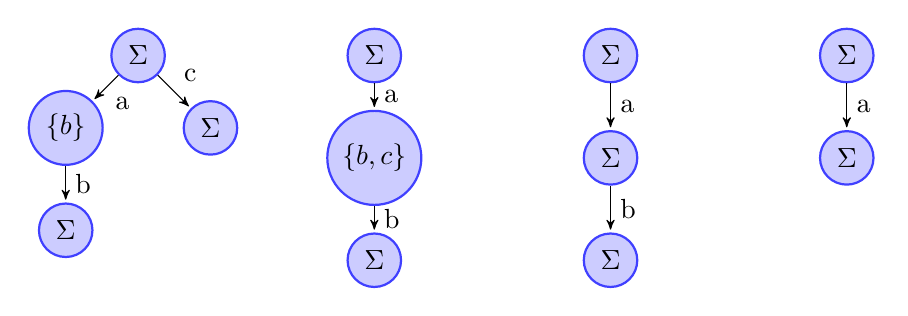
\begin{tikzpicture}[node distance=1.3cm,>=stealth',bend angle=45,auto]
  \tikzstyle{place}=[circle,thick,draw=blue!75,fill=blue!20,minimum size=6mm]
  \tikzstyle{red place}=[place,draw=red!75,fill=red!20]
  \tikzstyle{transition}=[rectangle,thick,draw=black!75,
  			  fill=black!20,minimum size=4mm]
  \tikzstyle{every label}=[red]
  \begin{scope}[xshift=0cm]
    \node [place] (w1) {$\Sigma$};
    \node [place] (e1) [below left of=w1] {$\{b\}$}
      edge [pre]  node[swap] {a}                 (w1);      
    \node [place] (c) [below of=e1] {$\Sigma $}
      edge [pre]  node[swap] {b}                 (e1);      
    \node [place] (e2) [below right of=w1] {$\Sigma $}
      edge [pre]  node[swap] {c}                 (w1);      
  \end{scope}  
  
  \begin{scope}[xshift=3cm]
    \node [place] (w1) {$\Sigma $};
    \node [place] (e1) [below of=w1] {$\{b,c\}$}
      edge [pre]  node[swap] {a}                 (w1);      
    \node [place] (e2) [below of=e1] {$\Sigma $}
      edge [pre]  node[swap] {b}                 (e1);      
  \end{scope}  
  
  \begin{scope}[xshift=6cm]
    \node [place] (w1) {$\Sigma $};
    \node [place] (e1) [below of=w1] {$\Sigma $}
      edge [pre]  node[swap] {a}                 (w1);      
    \node [place] (e2) [below of=e1] {$\Sigma $}
      edge [pre]  node[swap] {b}                 (e1);      
  \end{scope}  
  
  \begin{scope}[xshift=9cm]
    \node [place] (w1) {$\Sigma $};
    \node [place] (e1) [below of=w1] {$\Sigma $}
      edge [pre]  node[swap] {a}                 (w1);      
  \end{scope}  
  
  \draw (2,0) node {$\MODELLEQ $};
  \draw (4.5,0) node {$\MODELLEQ $};
  \draw (7.5,0) node {$\MODELLEQ $};
  
\end{tikzpicture}
\caption{Examples of $\MODELLEQ $}\label{figure:leq}
\end{FIGURE}


\end{frame}

\begin{frame}
\begin{figure}[H]
\centering
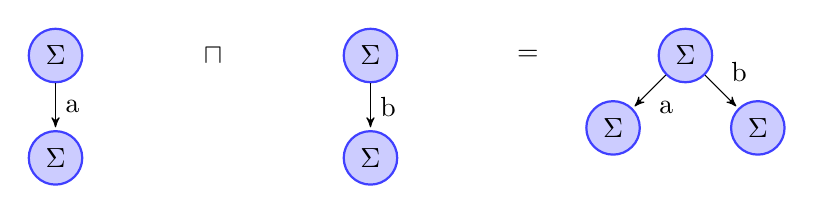
\begin{tikzpicture}[node distance=1.3cm,>=stealth',bend angle=45,auto]
  \tikzstyle{place}=[circle,thick,draw=blue!75,fill=blue!20,minimum size=6mm]
  \tikzstyle{red place}=[place,draw=red!75,fill=red!20]
  \tikzstyle{transition}=[rectangle,thick,draw=black!75,
  			  fill=black!20,minimum size=4mm]
  \tikzstyle{every label}=[red]
  \begin{scope}
    \node [place] (w1) {$\Sigma$};
    \node [place] (e1) [below of=w1] {$\Sigma$}
      edge [pre]  node[swap] {a}                 (w1);      
  \end{scope}
  \begin{scope}[xshift=4cm]
    \node [place] (w1) {$\Sigma$};
    \node [place] (e1) [below of=w1] {$\Sigma$}
      edge [pre]  node[swap] {b}                 (w1);      
  \end{scope} 
  \begin{scope}[xshift=8cm]
    \node [place] (w1) {$\Sigma$};
    \node [place] (e1) [below left of=w1] {$\Sigma$}
      edge [pre]  node[swap] {a}                 (w1);      
    \node [place] (e1) [below right of=w1] {$\Sigma$}
      edge [pre]  node[swap] {b}                 (w1);      
  \end{scope}
  \draw (2,0) node {$\sqcap$};
  \draw (6,0) node {$=$};
\end{tikzpicture}
\caption{Example of $\sqcap$.}
\end{figure}

\begin{figure}[H]
\centering
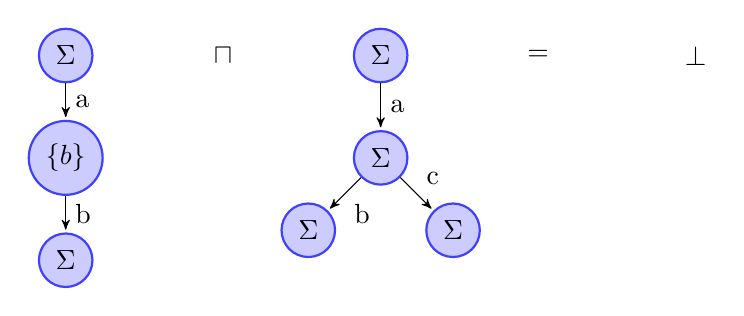
\begin{tikzpicture}[node distance=1.3cm,>=stealth',bend angle=45,auto]
  \tikzstyle{place}=[circle,thick,draw=blue!75,fill=blue!20,minimum size=6mm]
  \tikzstyle{red place}=[place,draw=red!75,fill=red!20]
  \tikzstyle{transition}=[rectangle,thick,draw=black!75,
  			  fill=black!20,minimum size=4mm]
  \tikzstyle{every label}=[red]
  \begin{scope}
    \node [place] (w1) {$\Sigma$};
    \node [place] (e1) [below of=w1] {$\{b\}$}
      edge [pre]  node[swap] {a}                 (w1);      
    \node [place] (e2) [below of=e1] {$\Sigma$}
      edge [pre]  node[swap] {b}                 (e1);      
  \end{scope}
  \begin{scope}[xshift=4cm]
    \node [place] (w1) {$\Sigma$};
    \node [place] (e1) [below of=w1] {$\Sigma$}
      edge [pre]  node[swap] {a}                 (w1);      
    \node [place] (e2) [below right of=e1] {$\Sigma$}
      edge [pre]  node[swap] {c}                 (e1);      
    \node [place] (e3) [below left of=e1] {$\Sigma$}
      edge [pre]  node[swap] {b}                 (e1);      
  \end{scope} 
  \begin{scope}[xshift=8cm]
    \node (w1) {$\bot$};
  \end{scope}
  \draw (2,0) node {$\sqcap$};
  \draw (6,0) node {$=$};
\end{tikzpicture}
\caption{Example of $\sqcap$.}
\end{figure}

\begin{figure}[H]
\centering
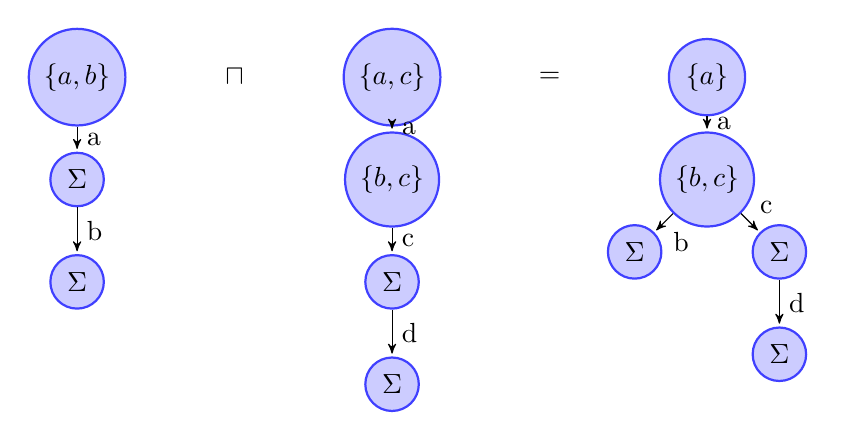
\begin{tikzpicture}[node distance=1.3cm,>=stealth',bend angle=45,auto]
  \tikzstyle{place}=[circle,thick,draw=blue!75,fill=blue!20,minimum size=6mm]
  \tikzstyle{red place}=[place,draw=red!75,fill=red!20]
  \tikzstyle{transition}=[rectangle,thick,draw=black!75,
  			  fill=black!20,minimum size=4mm]
  \tikzstyle{every label}=[red]
  \begin{scope}
    \node [place] (w1) {$\{a,b\}$};
    \node [place] (e1) [below of=w1] {$\Sigma$}
      edge [pre]  node[swap] {a}                 (w1);      
    \node [place] (e2) [below of=e1] {$\Sigma $}
      edge [pre]  node[swap] {b}                 (e1);      
  \end{scope}
  \begin{scope}[xshift=4cm]
    \node [place] (w1) {$\{a,c\}$};
    \node [place] (e1) [below of=w1] {$\{b,c\}$}
      edge [pre]  node[swap] {a}                 (w1);      
    \node [place] (e2) [below of=e1] {$\Sigma $}
      edge [pre]  node[swap] {c}                 (e1);      
    \node [place] (e3) [below of=e2] {$\Sigma $}
      edge [pre]  node[swap] {d}                 (e2);      
  \end{scope} 
  \begin{scope}[xshift=8cm]
    \node [place] (w1) {$\{a\}$};
    \node [place] (e1) [below of=w1] {$\{b, c\} $}
      edge [pre]  node[swap] {a}                 (w1);      
    \node [place] (e2) [below left of=e1] {$\Sigma $}
      edge [pre]  node[swap] {b}                 (e1);      
    \node [place] (e3) [below right of=e1] {$\Sigma $}
      edge [pre]  node[swap] {c}                 (e1);      
    \node [place] (e4) [below of=e3] {$\Sigma $}
      edge [pre]  node[swap] {d}                 (e3);      
  \end{scope}
  \draw (2,0) node {$\sqcap$};
  \draw (6,0) node {$=$};
\end{tikzpicture}
\caption{Example of $\sqcap$. }
\end{figure}

\begin{figure}[H]
\centering
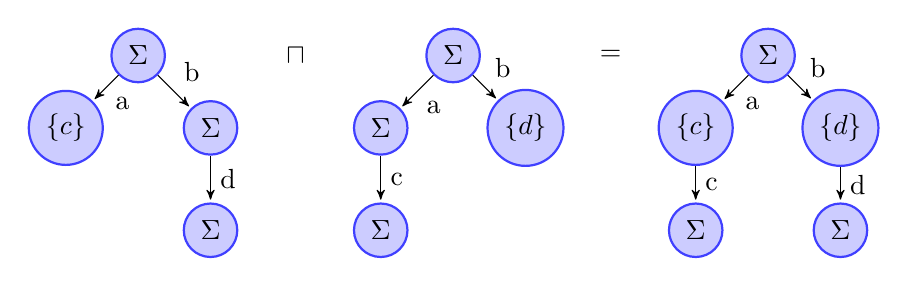
\begin{tikzpicture}[node distance=1.3cm,>=stealth',bend angle=45,auto]
  \tikzstyle{place}=[circle,thick,draw=blue!75,fill=blue!20,minimum size=6mm]
  \tikzstyle{red place}=[place,draw=red!75,fill=red!20]
  \tikzstyle{transition}=[rectangle,thick,draw=black!75,
  			  fill=black!20,minimum size=4mm]
  \tikzstyle{every label}=[red]
  
  \begin{scope}
    \node [place] (w1) {$\Sigma$};
    \node [place] (e1) [below left of=w1] {$\{c\}$}
      edge [pre]  node[swap] {a}                 (w1);      
    \node [place] (e2) [below right of=w1] {$\Sigma$}
      edge [pre]  node[swap] {b}                 (w1);      
    \node [place] (e3) [below of=e2] {$\Sigma$}
      edge [pre]  node[swap] {d}                 (e2);      
  \end{scope}
  
  \begin{scope}[xshift=4cm]
    \node [place] (w1) {$\Sigma$};
    \node [place] (e1) [below left of=w1] {$\Sigma$}
      edge [pre]  node[swap] {a}                 (w1);      
    \node [place] (e2) [below right of=w1] {$\{d\}$}
      edge [pre]  node[swap] {b}                 (w1);      
    \node [place] (e3) [below of=e1] {$\Sigma$}
      edge [pre]  node[swap] {c}                 (e1);      
  \end{scope}
  
  
  \begin{scope}[xshift=8cm]
    \node [place] (w1) {$\Sigma$};
    \node [place] (e1) [below left of=w1] {$\{c\}$}
      edge [pre]  node[swap] {a}                 (w1);      
    \node [place] (e2) [below right of=w1] {$\{d\}$}
      edge [pre]  node[swap] {b}                 (w1);      
    \node [place] (e3) [below of=e1] {$\Sigma$}
      edge [pre]  node[swap] {c}                 (e1);      
    \node [place] (e4) [below of=e2] {$\Sigma$}
      edge [pre]  node[swap] {d}                 (e2);      
  \end{scope}
  
  \draw (2,0) node {$\sqcap$};
  \draw (6,0) node {$=$};
\end{tikzpicture}
\caption{Example of $\sqcap$.}
\end{figure}


\end{frame}

\begin{frame}
\begin{figure}[H]
\centering
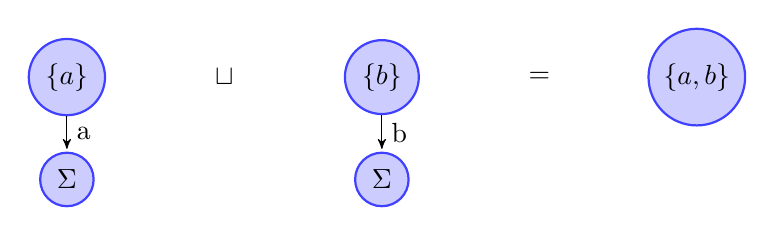
\begin{tikzpicture}[node distance=1.3cm,>=stealth',bend angle=45,auto]
  \tikzstyle{place}=[circle,thick,draw=blue!75,fill=blue!20,minimum size=6mm]
  \tikzstyle{red place}=[place,draw=red!75,fill=red!20]
  \tikzstyle{transition}=[rectangle,thick,draw=black!75,
  			  fill=black!20,minimum size=4mm]
  \tikzstyle{every label}=[red]
  \begin{scope}
    \node [place] (w1) {$\{a\}$};
    \node [place] (e1) [below of=w1] {$\Sigma$}
      edge [pre]  node[swap] {a}                 (w1);      
  \end{scope}
  \begin{scope}[xshift=4cm]
    \node [place] (w1) {$\{b\}$};
    \node [place] (e1) [below of=w1] {$\Sigma$}
      edge [pre]  node[swap] {b}                 (w1);      
  \end{scope}
  \begin{scope}[xshift=8cm]
    \node [place] (w1) {$\{a,b\}$};
  \end{scope}
  \draw (2,0) node {$\sqcup$};
  \draw (6,0) node {$=$};
\end{tikzpicture}
\caption{Example of $\sqcup$}
\end{figure}


\begin{figure}[H]
\centering
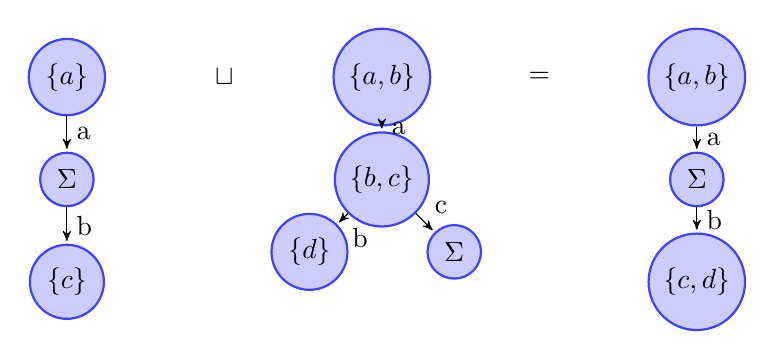
\begin{tikzpicture}[node distance=1.3cm,>=stealth',bend angle=45,auto]
  \tikzstyle{place}=[circle,thick,draw=blue!75,fill=blue!20,minimum size=6mm]
  \tikzstyle{red place}=[place,draw=red!75,fill=red!20]
  \tikzstyle{transition}=[rectangle,thick,draw=black!75,
  			  fill=black!20,minimum size=4mm]
  \tikzstyle{every label}=[red]
  \begin{scope}
    \node [place] (w1) {$\{a\}$};
    \node [place] (e1) [below of=w1] {$\Sigma$}
      edge [pre]  node[swap] {a}                 (w1);      
    \node [place] (e2) [below of=e1] {$\{c\}$}
      edge [pre]  node[swap] {b}                 (e1);      
  \end{scope}
  \begin{scope}[xshift=4cm]
    \node [place] (w1) {$\{a,b\}$};
    \node [place] (e1) [below of=w1] {$\{b,c\}$}
      edge [pre]  node[swap] {a}                 (w1);      
    \node [place] (e2) [below left of=e1] {$\{d\}$}
      edge [pre]  node[swap] {b}                 (e1);      
    \node [place] (e2) [below right of=e1] {$\Sigma$}
      edge [pre]  node[swap] {c}                 (e1);      
  \end{scope} 
  \begin{scope}[xshift=8cm]
    \node [place] (w1) {$\{a,b\}$};
    \node [place] (e1) [below of=w1] {$\Sigma$}
      edge [pre]  node[swap] {a}                 (w1);      
    \node [place] (e2) [below of=e1] {$\{c,d\}$}
      edge [pre]  node[swap] {b}                 (e1);      
  \end{scope}
  \draw (2,0) node {$\sqcup$};
  \draw (6,0) node {$=$};
\end{tikzpicture}
\caption{Example of $\sqcup$}
\end{figure}

\end{frame}


\begin{frame}{Inference Rules}
\begin{FIGURE}
\begin{RULES}

  \ZEROPREMISERULENAMEDRIGHT
  {
    \phi \judge \phi
  }{Identity}
    \quad
  \ZEROPREMISERULENAMEDRIGHT
  {
    \phi \judge \top
  }{$\top$-Right}
    \quad
  \ZEROPREMISERULENAMEDRIGHT
  {
    \bot \judge \phi
  }{$\bot$-Left}
    \quad
  \TWOPREMISERULENAMEDRIGHT
  {
    \phi \judge \psi
  }
  {
    \psi \judge \xi
  }
  {
    \phi \judge \xi
  }{Transitivity}
    \\\\
  \ONEPREMISERULENAMEDRIGHT
  {
    \phi \judge \psi
  }
  {
    \phi \AND \xi \judge \psi
  }{$\AND$-Left 1}
     \quad
  \ONEPREMISERULENAMEDRIGHT
  {
    \phi \judge \psi
  }
  {
    \xi \AND \phi  \judge \psi
  }{$\AND$-Left 2}
     \quad
  \TWOPREMISERULENAMEDRIGHT
  {
    \phi \judge \psi
  }
  {
    \phi \judge \xi
  }
  {
    \phi \judge \psi \AND \xi
  }{$\AND$-Right}
     \\\\
     \ONEPREMISERULENAMEDRIGHT
     {
       a \notin A
     }
     {
       !A \AND \MAY{a}{\phi} \judge \bot
     }{$\bot$-Right 1}
        \quad
     \ZEROPREMISERULENAMEDRIGHT
     {
       \MAY{a}{\bot} \judge \bot
     }{$\bot$-Right 2}
        \quad
     \TWOPREMISERULENAMEDRIGHT
     {
       \phi \AND \, !A \judge \psi
     }
     {
       A' \subseteq A
     }
     {
       \phi \AND\, !A' \judge \psi
     }{!-Left}
     \\\\
     \TWOPREMISERULENAMEDRIGHT
     {
       \phi \judge !A
     }
     {
       A \subseteq A'
     }
     {
       \phi \judge!A'
     }{!-Right 1}
     \quad
     \TWOPREMISERULENAMEDRIGHT
     {
       \phi \judge !A
     }
     {
       \phi \judge !B
     }
     {
       \phi \judge !(A \cap B)
     }{!-Right 2}
     \quad
     \ONEPREMISERULENAMEDRIGHT
     {
       \phi \judge \psi
     }
     {
       \MAY{a}{\phi} \judge \MAY{a}{\psi}
     }{Transition Normal}
\end{RULES}
\caption{Proof rules.}\label{figure:elAndBangRules}
\end{FIGURE}

\end{frame}

\begin{frame}
\begin{FIGURE}
\begin{RULES}
     \ONEPREMISERULENAMEDRIGHT
     {
       a \notin A
     }
     {
       !A \AND \MAY{a}{\phi} \judge \bot
     }{$\bot$-Right 1}
        \qquad
     \ZEROPREMISERULENAMEDRIGHT
     {
       \MAY{a}{\bot} \judge \bot
     }{$\bot$-Right 2}
     \\\\
     \TWOPREMISERULENAMEDRIGHT
     {
       \phi \judge !A
     }
     {
       A \subseteq A'
     }
     {
       \phi \judge!A'
     }{!-Right 1}
     \qquad
     \TWOPREMISERULENAMEDRIGHT
     {
       \phi \judge !A
     }
     {
       \phi \judge !B
     }
     {
       \phi \judge !(A \cap B)
     }{!-Right 2}
     \\\\
     \ONEPREMISERULENAMEDRIGHT
     {
       \phi \judge \psi
     }
     {
       \MAY{a}{\phi} \judge \MAY{a}{\psi}
     }{Normal}
     \qquad
     \ONEPREMISERULENAMEDRIGHT
     {
       \phi \judge \MAY{a}\psi \land \MAY{a}\xi
     }
     {
       \phi \judge \MAY{a}(\psi \land \xi)
     }{Det}
\end{RULES}
\caption{Proof rules.}\label{figure:elAndBangRules}
\end{FIGURE}

\end{frame}

\begin{frame}
Theorem 5: The rules are sound and complete
\end{frame}

\begin{frame}
Other stuff:
\begin{itemize}
\item
Translation from \cathoristic{} to first-order logic
\item
Proof of compactness
\item
\Cathoristic{} satisfies Brandom's Incompatibility Semantics property: $\phi \models \psi$ iff $\mathcal{I}(\psi) \subseteq \mathcal{I}(\phi)$
\item
\Cathoristic{} with negation
\item
Quantified \cathoristic{}
\end{itemize}
\end{frame}

\begin{frame}{Open problems}

  Many, but crucial: what are the properties of negation when defined
  on top of exclusion?

  \VSPACE\pause

  How can we use this in program verification? It 'feels' useful ...
  
\end{frame}

\begin{frame}
What does this all have to do with Chris?
\end{frame}

\begin{frame}
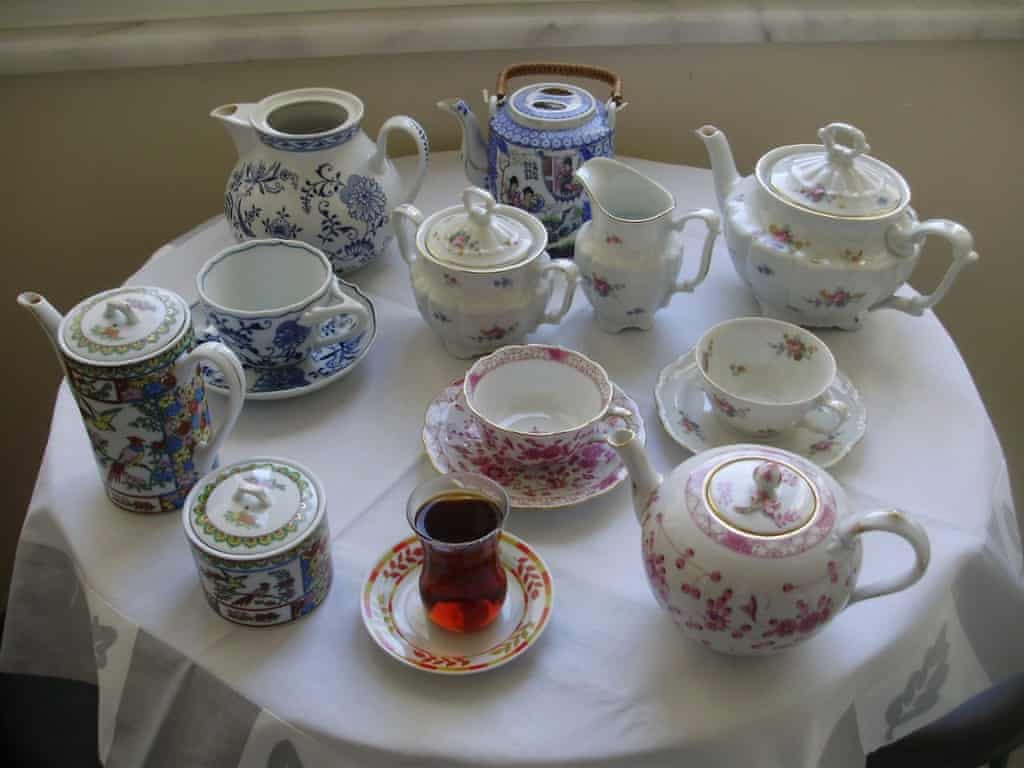
\includegraphics[height=9cm]{images/tea.jpeg}
\end{frame}

\begin{frame}

\includegraphics[height=9cm]{images/rave.jpg}
\end{frame}

\begin{frame}
Thanks Chris!
\end{frame}



\end{document}


\end{document}
